
\documentclass[conference]{IEEEtran}
\usepackage{blindtext, graphicx, amsmath, todonotes}

\hyphenation{net-works}

\begin{document}

\title{Modeling Heterogeneous Traffic Performance with the 802.11 DCF}

\author{\IEEEauthorblockN{Tamir Husain and Christopher A. Wood}
\IEEEauthorblockA{Department of Computer Science\\
University of California Irvine\\
Email: thusain@uci.edu, woodc1@uci.edu}
% \and
% \IEEEauthorblockN{name}
% \IEEEauthorblockA{Twentieth Century Fox\\
% Springfield, USA\\
% Email: homer@thesimpsons.com}
}

% make the title area
\maketitle

\begin{abstract}
%\boldmath
% TODO
\end{abstract}

\begin{IEEEkeywords}
% TODO
\end{IEEEkeywords}

\IEEEpeerreviewmaketitle

\section{Introduction}
Wireless networks have become pervasive in modern computer and communication systems. The widespread adoption of mobile and personal computing devices, such as smartphones and tablets, continues to drive commercial investment in high performance wireless networking technologies. Concurrently, the type of traffic traversing these networks has also evolved -- divergently -- an increasing rate. Every kind of information from textual data to video stream segments traverse wireless networks. Society's dependence on WLAN technologies like the 802.11 MAC and PHY protocol suites have cultivated a massive amount of analytical and experimental research studying their performance. 

\todo[inline]{Come back later...}
A major portion of this research has focused on the 802.11 distributed control function (DCF). In particular, there is a lack of analytical analysis studying the performance of heterogeneous traffic in a multi-node system. We address this gap.

\section{Related Work}
% \cite{dcf}
% \cite{dcf-nonsaturated}
% TODO


%%% simulation papers
% bianchi1998ieee
% bianchi1996performance
% crow1996performance
% chhaya1997performance

\section{Heterogeneous Traffic Models}
Today's computer and communication networks are being used to transfer increasingly heterogeneous traffic between parties. In particular, file downloads, standard web browsing, video streaming, and client-server video game traffic are four very common types of traffic that dominate the Internet traffic today. In this section, we describe the characteristics of each of these traffic types. We use a variety of parameters to describe these types of traffic. Specifically, we focus on packet size, interrival time, traffic saturation, and burstiness. 

\begin{itemize}
	\item File Download Traffic: A model for file downloads must support long bursts of packet arrivals and long interarrival times. 

	\item Web Browsing Traffic: Web browsing traffic is quite diverse in packet size, interrarival time, and burstiness. For simplicity, we assume that web browsing traffic has uniform packet sizes, deterministic interarrival time, and probabilistic packet arrival in the buffer. This enables us to use the nonsaturated DCF model to study this traffic.

	\item Video Streaming Traffic: Video streaming traffic as described in \cite{badia2010markov} is composed of two types of packets -- I and D packets -- each of which are tightly correlated and with different characteristics. Video segments are sent in sets of I and D packets, wherein multiple small D packets carrying video data are dependent on a single I packet with metadata necessary to decode the video stream. The length of each I and D packet is correlated to past packet lengths. For example, let $\lambda_j(t|s)$ denote the probability that a packet of type $j \in \{I ,D \}$ is $t$ time slots long given that the previous packet of type $j$ was $s$ packets long. The size of both I and D packets are bounded within a finite range so as to make the analytical model tractable. 

	\item Client-Server Video Game Traffic: Branch et al. \cite{branch2008markov} showed that client-server video game traffic, particularly that of first-person shooters, has characteristics consistent with a subclass of Markov models known as autoregressive model or order 1 (AR(1)). These time-series models have the form
	\begin{align*}
	y_0 & = \mu_0 \\
	y_{n+1} & = \beta y_n + Z_n, (n \geq 1),
	\end{align*}
	where $y_n$ are the discrete points in time, $\beta$ is a constant, and $Z_n, n \geq 1$, are i.i.d. variables. 
\end{itemize}

We will use the characteristics of each of these models to tune our analytical approach in the experimental section of this report. 

\section{The 802.11 Distributed Control Function}
The 802.11 DCF \cite{ieee1997wireless} is at the core of this work. It is a simplistic random access scheme based on the carrier sense multiple access with collision avoidance (CSMA/CA) protocol. Failed packets are retried according to a binary exponential backoff rule. At each packet transmission, the backoff is uniformly in the range ($0, w-1$), where $w$ is the length of the ``contention window'' and is directly dependent on the number of failed attempts for the packet thus far. The window $w$ is set to $W_{min}$ to begin, and upon every failure, the backoff counter is doubled. At stage $i$, the backoff timer is $2^iW_{min}$. The maximum backoff is bounded by $W_{max} = 2^mW_{min}$. Selections of $W_{min}$ and $W_{max}$ are dependent upon the physical layer specifications in the 802.11 standard \cite{ieee1997wireless,dcf}. For example, frequency hopping spread spectrum calls for $W_{min} = 16$ and $W_{max} = 1024$ ($m = 6$). 

\section{Incremental Markov Models for Heterogeneous Traffic}

\subsection{Original DCF Model}
A simple Markov model for the 802.11 DCF function was proposed in the seminal work by Bianchi \cite{dcf}. The system state is described by two discrete-time stochastic processes $b(t)$ and $s(t)$: $b(t)$ represents the backoff \emph{time counter} and $s(t)$ represents the backoff \emph{stage} for a given station or node, each of which is advanced at each time step (i.e., from $t$ to $t + 1$). Each node is equipped with a \emph{saturated} buffer of packets to transmit; there is never a case where a node has to wait for a packet to arrive in the buffer before attempting a transmission. Also, instead of modeling multiple nodes simultaneously to accurately assess the probability of collision, this model assumes a constant probability of collision $p$ -- the conditional collision probability -- at each time slot. In the real world, this probability is a function of the network and environmental interferences, e.g., shadowing, fading, etc. However, by making this a constant and therefore independent from other nodes, the model simplifies to capturing the dynamics of the bidimensional process $\{ b(t), s(t) \}$ as a discrete-time Markov chain, shown in Figure \ref{fig:dcf_model}. 

The only non-null transition probabilities in this Markov chain are given below:
\begin{math}
\boxed{
\begin{array}{lll}
\Pr[i,k | i, k + 1] = 1 & k \in [0, W_i - 2] & i \in [0,m] \\
\Pr[0,k | i, 0] = (1-p)/W_0 & k \in [0, W_0 - 1] & i \in [0,m] \\
\Pr[i,k | i-1, k] = p/W_i & k \in [0, W_i - 1] & i \in [1,m] \\
\Pr[m,k | m,0] = p/W_m & k \in [0, W_m - 1] & ~
\end{array}
}
\end{math}

\begin{figure*}
\begin{center}
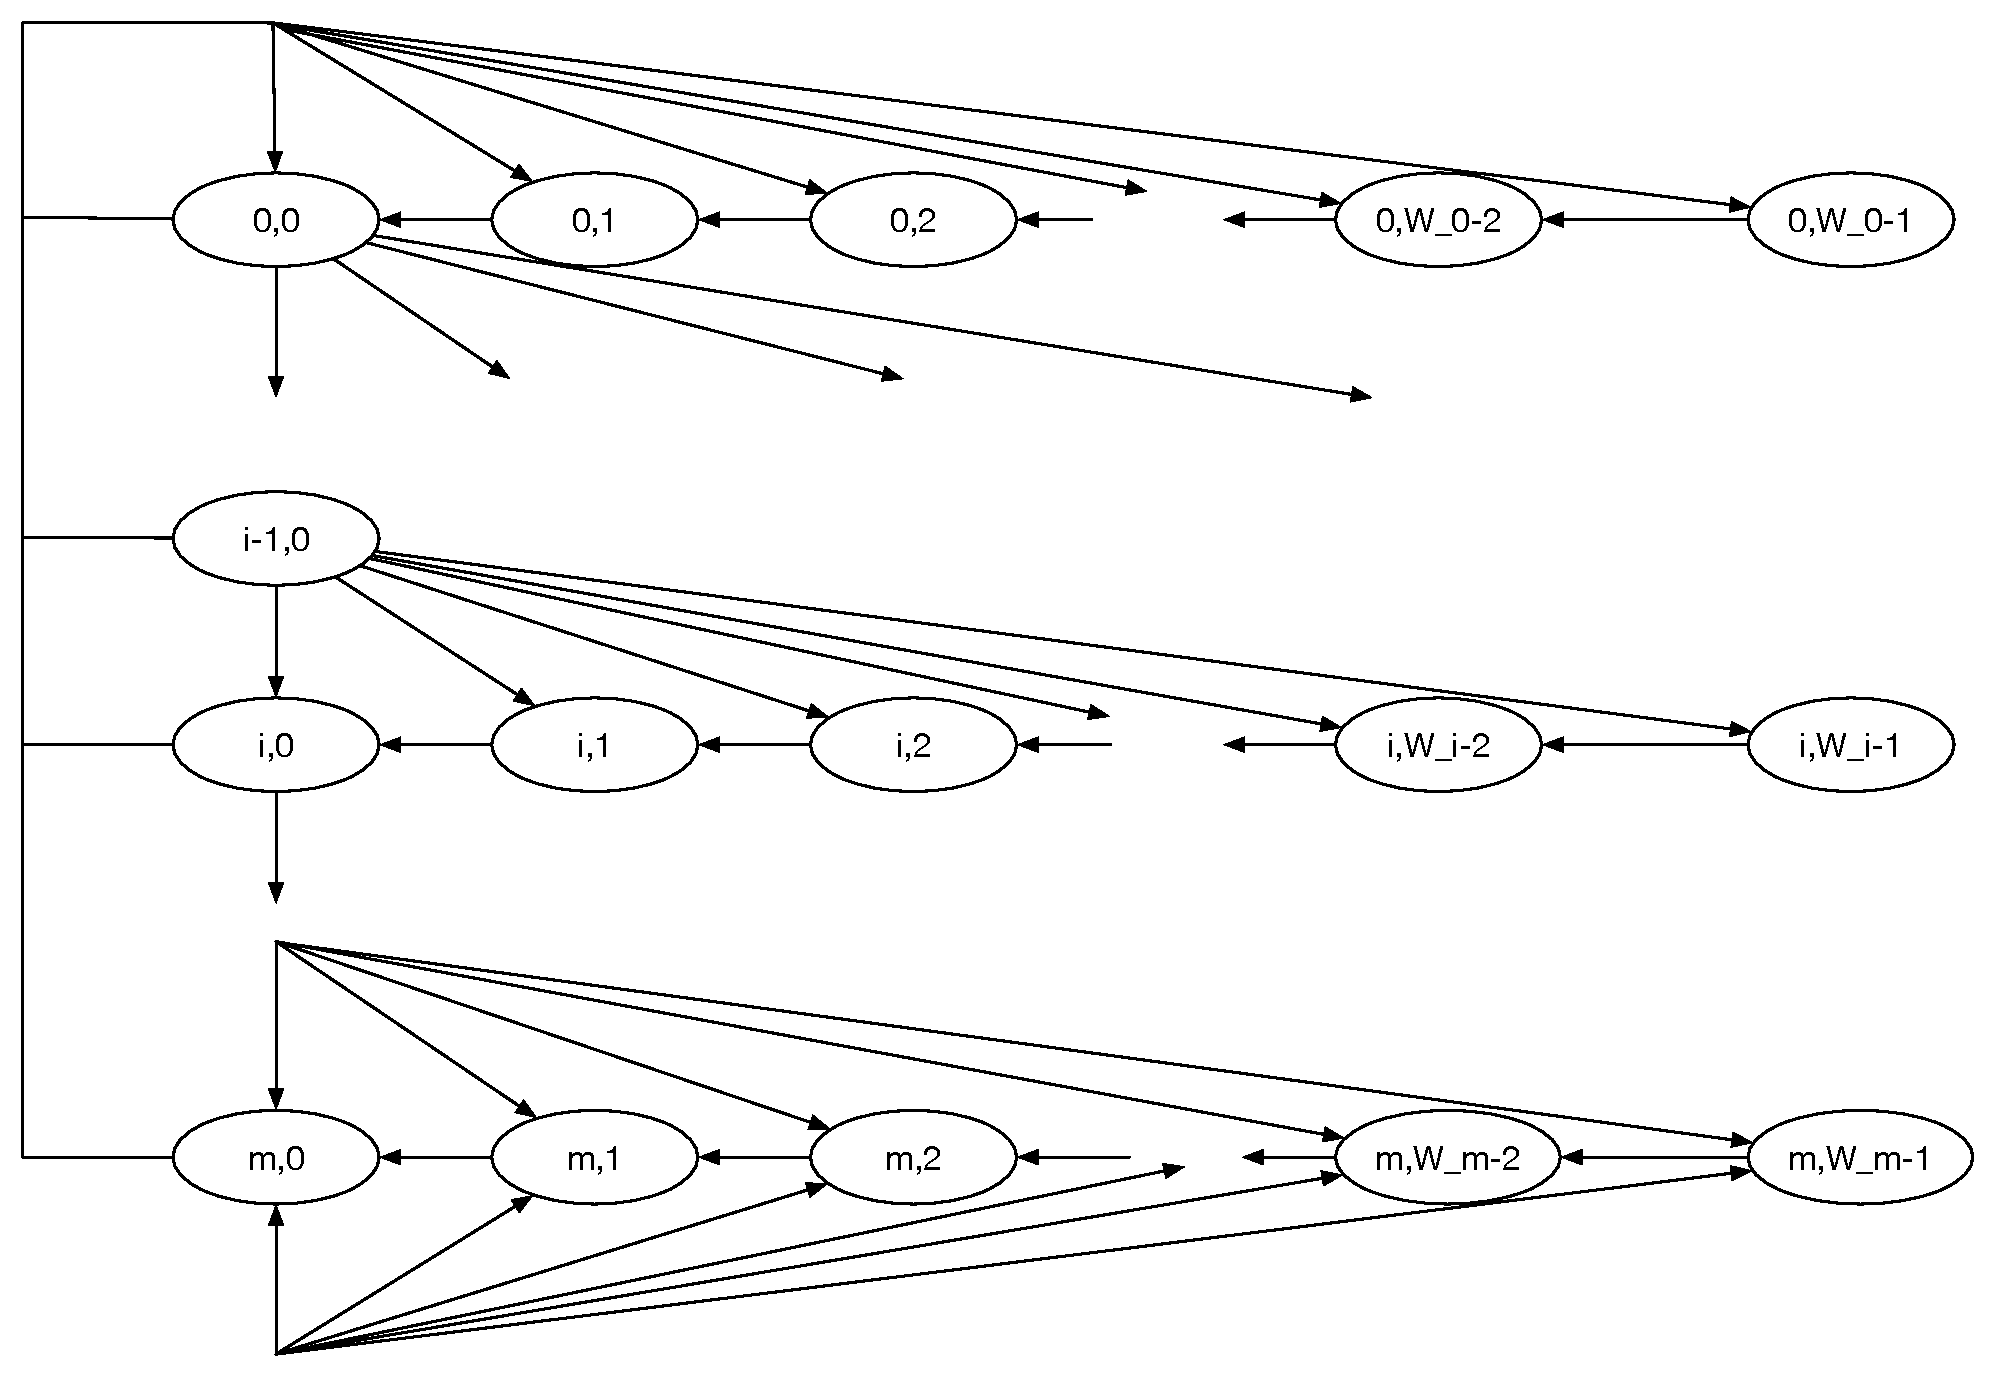
\includegraphics[scale=0.5]{../sketches/dcf_model.pdf}
\caption{The original saturated DCF Markov model \cite{dcf}.}
\label{fig:dcf_model}
\end{center}
\end{figure*}

\subsection{Limited and Diverse Traffic}
While accurate, the original DCF model is constrained in that it assumes homogeneous traffic and a saturated stream of packets for transmission. Malone et al. \cite{dcf-nonsaturated} presented a modified version of Bianchi's model that captures non-saturated traffic loads. The essential idea behind their variant is that there exists a constant packet arrival probability $q$ at each time slot, much like there exists a constant collision probability $p$. If a node successfully transmits a packet and the buffer is not-empty, the state of the system proceeds as normal. Conversely, if a packet is not ready for transmission, then the chain enters a stage known as ``postbackoff,'' denoted $(0,k)_e$ for $k \in [0, W_0-1]$. A node may state in this state indefinitely until a packet arrives. 

To capture the mechanics of the DCF function in this condition, the postbackoff set of stages are nearly indentical to backoff stage $i = 0$. If a packet arrives at any time when the system is in a postbackoff state, it immediately transitions into the backoff stage $i = 0$, with a decremented backoff timer. However, if the postbackoff timer reaches $0$, where the postbackoff is said to be complete, the node will stay in this state until a packet arrives with probability $q$. Once a packet arrives in state $(0, 0)_e$ with probability $q$, there are three possible outcomes: (1) the packet is transmitted successfully, a collision occurs with probability $p$, or the medium (channel) is sensed as busy with probability $1 - P_{idle} = p$. 

With the addition of the postbackoff states $S'$, the Markov chain itself is now a multidimensional process $\{b(t), s(t), S' \}$. The new state transition probabilities needed to capture the transitions between these multiple dimensions are below.
\begin{math}
\boxed{
\begin{array}{lll}
\Pr[(i,k-1) | (i, k)] = 1 & k \in [1, W_i-1] & i \in [1,m] \\
\Pr[(0,k-1)_e | (0, k)_e] = 1-q & k \in [1, W_i-1] & i \in [1,m] \\
\Pr[(0,k-1) | (0, k)_e] = q & k \in [1, W_i-1] & i \in [1,m] \\
\end{array}
}
\end{math}

\begin{math}
\boxed{
\begin{array}{lll}
\Pr[(0,k)_e | (i, 0)] = \frac{(1-p)(1-q)}{W_0} & k \geq 0 & i \in [0,m] \\
\Pr[(0,k) | (i, 0)] = \frac{(1-p)q}{W_0} & k \geq 0 & i \in [0,m] \\
\Pr[(\max\{(i+1,m\}, k) | (i, 0)] = \frac{p}{W_{\max\{i+1,m\}}} & k \geq 0 & i \in [0,m] \\
\end{array}
}
\end{math}

\begin{math}
\boxed{
\begin{array}{ll}
\Pr[(0,0)_e | (0, 0)_e] = 1 - q + \frac{qP_{idle}(1 - p)}{W_0} & ~ \\
\Pr[(0,k)_e | (0, 0)_e] = \frac{qP_{idle}(1 - p)}{W_0} & k > 0 \\
\Pr[(1,k) | (0, 0)_e] = \frac{qP_{idle}p}{W_1} & k \geq 0 \\
\Pr[(0,k) | (0, 0)_e] = \frac{q(1 - P_{idle})}{W_0} & k \geq 0 \\
\end{array}
}
\end{math}

\begin{figure*}
\begin{center}
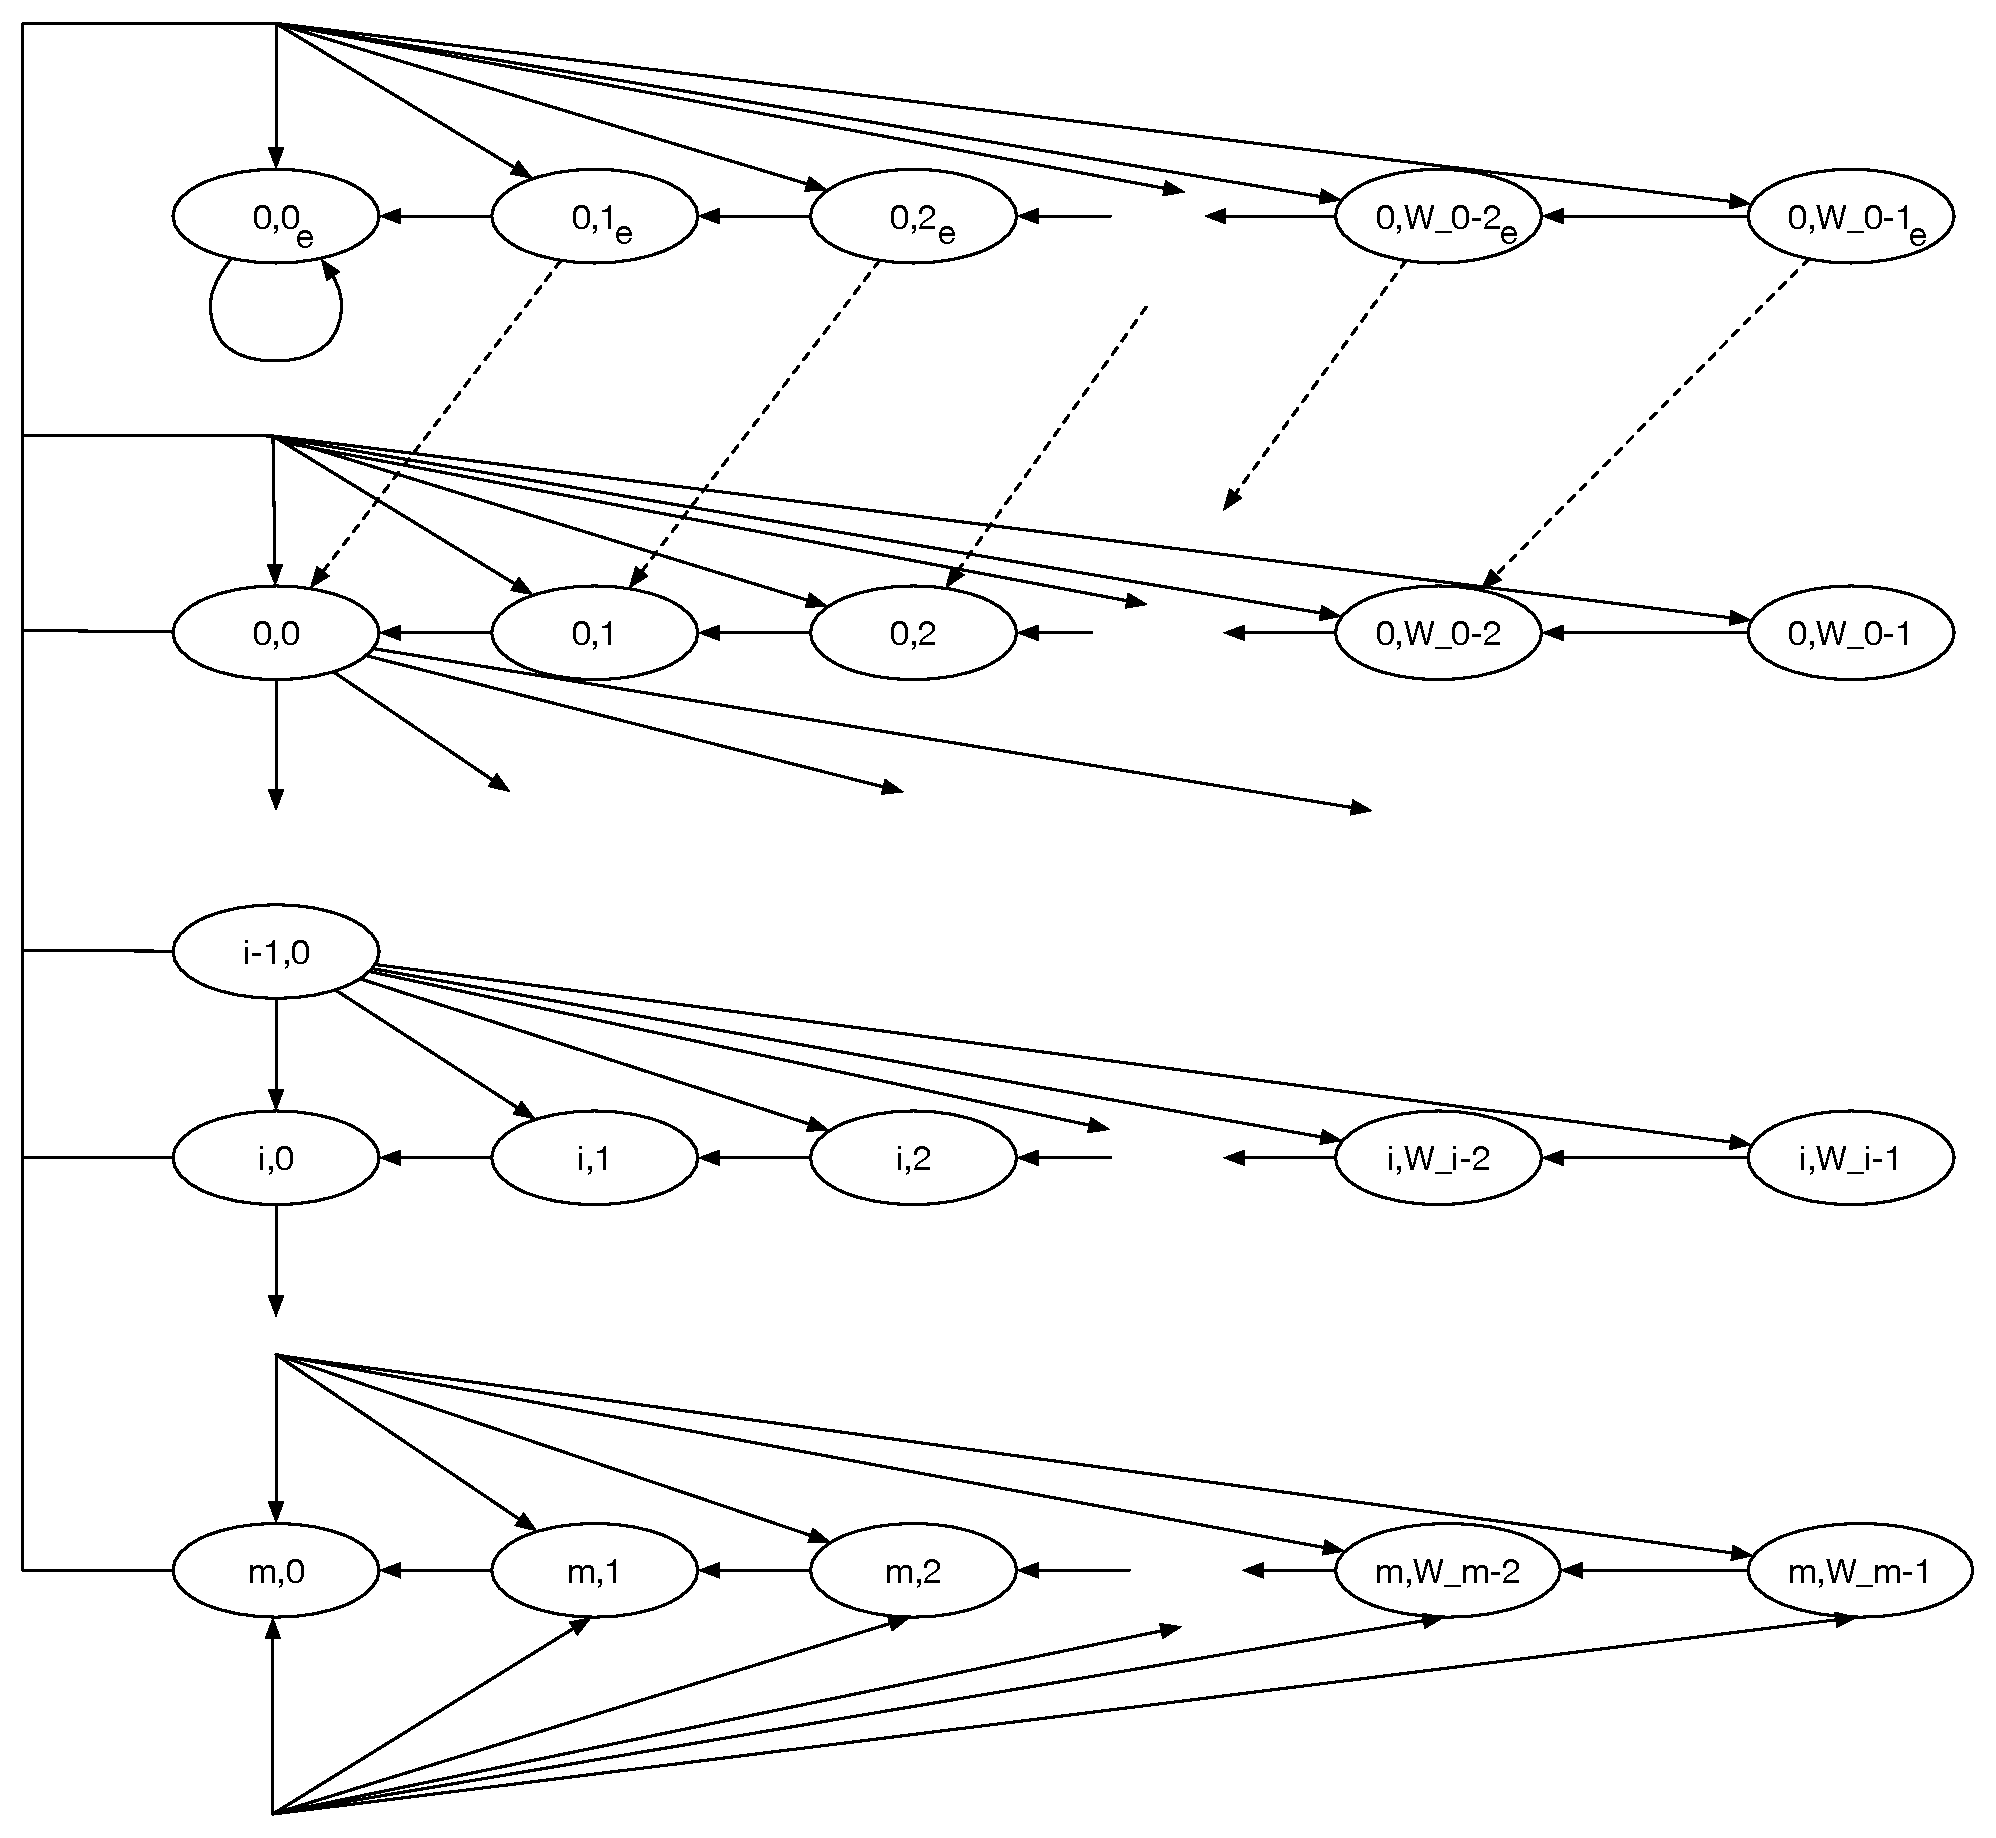
\includegraphics[scale=0.5]{../sketches/dcf_model_nonsaturated.pdf}
\caption{The modified DCF Markov model that captures non-saturated traffic \cite{dcf-unsaturated}.}
\label{fig:dcf_model_nonsaturated}
\end{center}
\end{figure*}

Malone et al. \cite{dcf-nonsaturated} exploited the inclusion of this postbackoff state and the fixed arrival probability constant to study the performance of the DCF while transferring packets from unsaturated heterogeneous traffic, e.g., file downloads, web traffic, etc.

\subsection{Adding Variable Length Frame Payloads}
Despite the flexibilty in the previous model, it is still limited with respect to packet size. In particular, the model assumes that each packet has an equally sized payload. This is not true, especially for video traffic \cite{???}, which typically consists of two types of packets of distinctly different sizes: $d$ packets are small video frame/segment packets that carry information needed to render a piece of video data, and $i$ packets are large ``metadata'' packets that contain information necessary to decode $d$ packets. Multiple $d$ packets are often tied to a single $i$ packet in such a way that if the $i$ packet is lost, none of its children $d$ packets can be decoded correctly. Consequently, we need to be able to model packets of different sizes. 

To do this, we consider a range of possible packet sizes, e.g., $[1,l]$, where $l$ is the maximum packet payload size. In this context, the packet size corresponds to \emph{how many} discrete time slots are needed to transfer the content over the channel. In the previously two discussed models, the packet size was assumed to be $1$ since they were assumed to be transferred in a single time step. Since we may want to support both deterministic and arbitrary packet sizes, drawn from a specific distribution, we use what we call size chain blackboxes to capture this type of variability. Figure \ref{fig:size_chain} shows a sample size chain blackbox for the range of values $[1,4]$. There are $l$ ($l = 4$) transitions into the blackbox, and each transition $l'$ is to a chain of length $l'$. 

\begin{figure}
\begin{center}
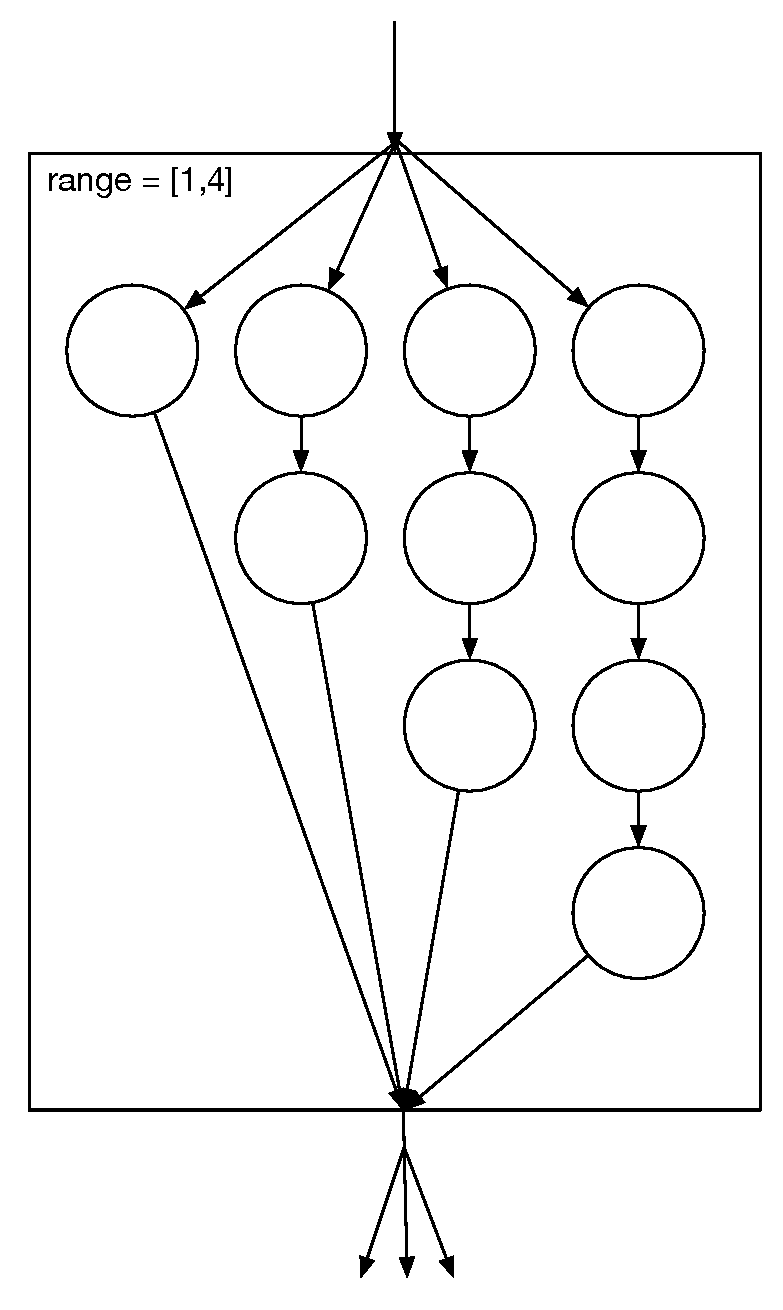
\includegraphics[scale=0.4]{../sketches/size_chain_old.pdf}
\caption{A blackbox Markov chain that captures bounded variabilities in a particular parameter, such as packet length or packet interarrival time.}
\label{fig:size_chain}
\end{center}
\end{figure}

To show how this chain would be used, assume that the size chain blackbox represents the size of a particulr packet. Further, assume that the packet size is a discrete random variable ranging from 1 to 4 with uniform distribution. The probability of transferring to any chain within the blackbox from the entry state is $(1/4)$. If the transition was to the last chain of length $l = 4$, then the state would appear to ``loop'' in place for 4 time steps before exiting the blackbox. Conversely, if the transition was to the first chain of length $l = 1$, then the state would only loop once before exiting. Although these states are costly from the persepctive of space, this type of construction enables us to model such discrete random variables with any distribution within our Markov chain. 

The first application of these size chain blackboxes are to extend the previously discusssed nonsaturated model to support variable packet sizes. Specifically, the number of time steps needed to transfer a packet and detect collision is now a bounded discrete random variable. This means that once a packet has begin transmitting it enters a size chain blackbox before either (a) detecting collision or (b) completing successfully. It is important to note that for packets of length $l > 1$, the probability of a collision is no longer $q$. Rather, a collision occurs if there is a collision in \emph{any} time slot during which the packet was being transmitted. This means that the probability of collision for a packet of length $l$ is $1 - (1 - p)^l$. 

The new states required to model the size chain blackboxes are tuples of the form $(i, l, l')$, where $i$ is the backoff stage and $l$ is the packet length, and $l'$ is the \emph{state} within the size chain of length $l$. For example, if the state transitions into a size chain of length $l = 4$ from state $(i, 0)$, then the following series of transitions would occur: 
\begin{align*}
(i, 4, 4) & \to (i, 4, 3) \\
& \to (i, 4, 2) \\
& \to (i, 4, 1)
\end{align*}

To model this behavior, which is visually shown in Figure \ref{fig:dcf_model_unsaturated_varpktsize}, the following new state transition probabilities are included into the model:
\begin{math}
\boxed{
\begin{array}{lll}
\Pr[(i,l,l'-1) | (i,l,l')] = 1 & l' \leq l & l' \geq 0 \\
\Pr[(i+1,k) | (i,l,0)] = \frac{1 - (1 - p)^l}{W_{i+1}} & ~ & k \in (0, W_{i+1} - 1) \\
\Pr[(0,k) | (i,l,0)] = \frac{(1 - q)(1 - p)^l}{W_0} & ~ & k \in (0, W_{0} - 1) \\
\Pr[(0,k)_e | (i,l,0)] = \frac{q(1 - p)^l}{W_0} & ~ & k \in (0, W_{0} - 1) \\
\end{array}
}
\end{math}

\begin{figure*}
\begin{center}
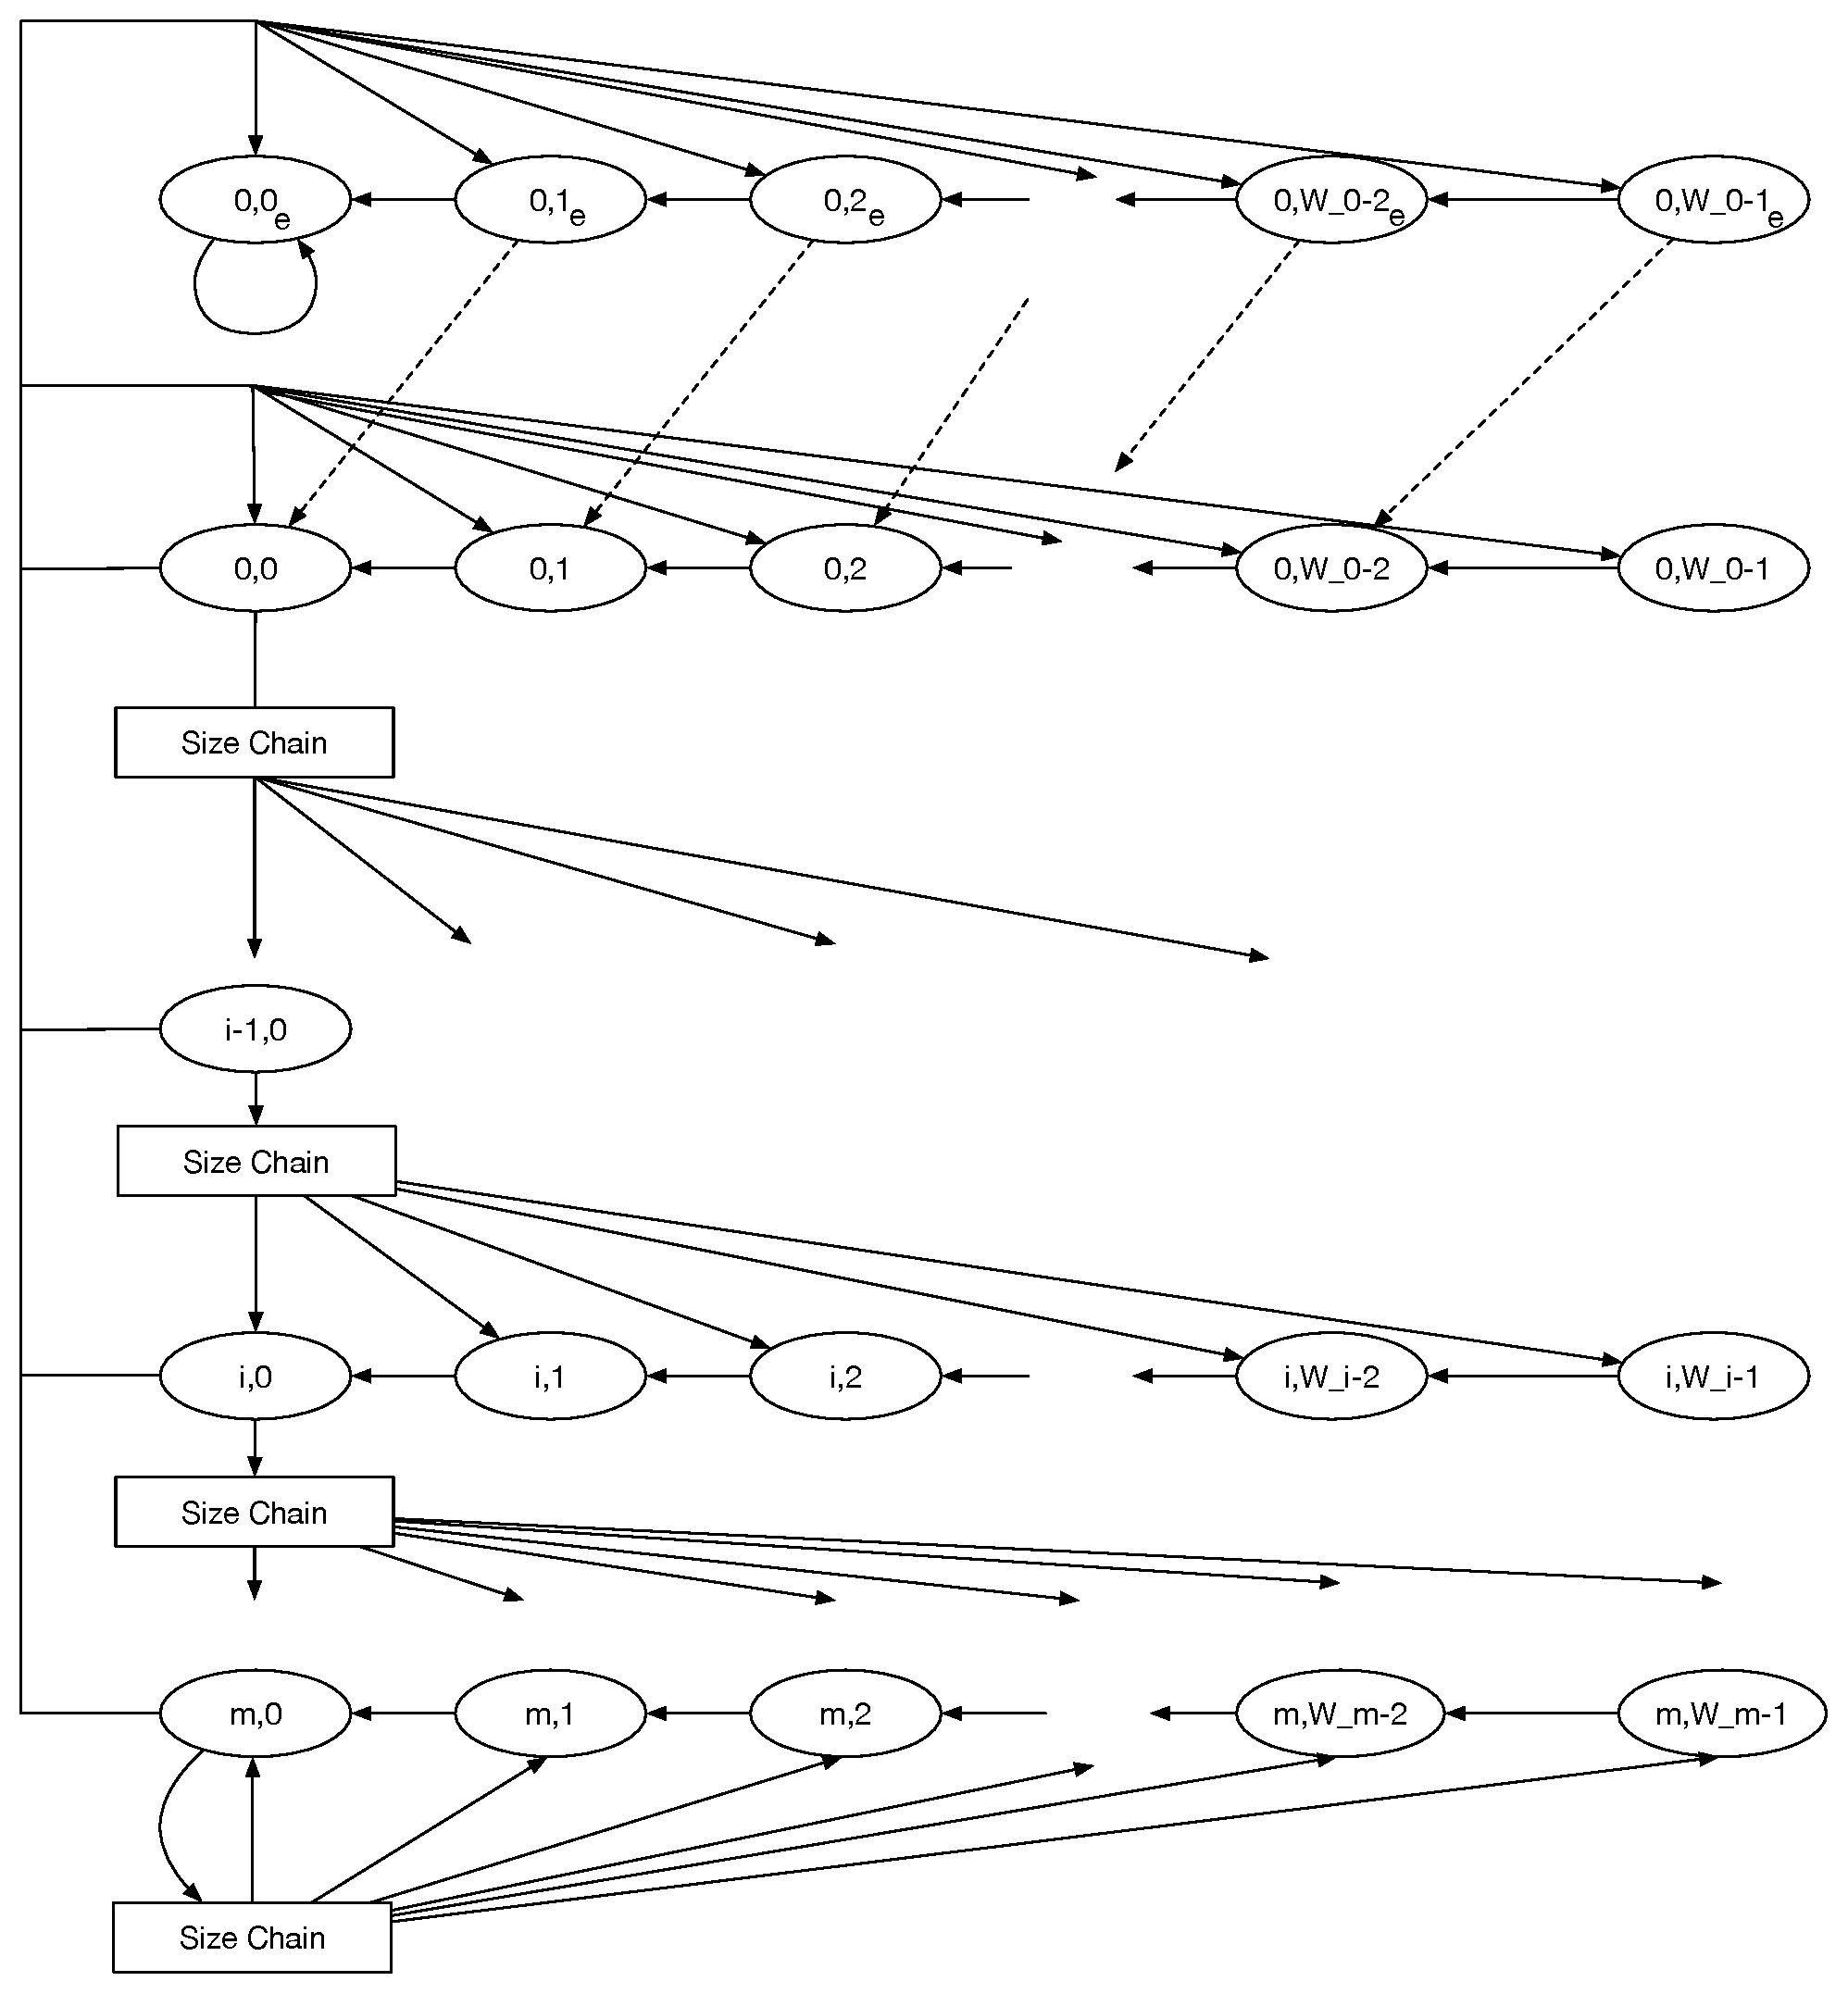
\includegraphics[scale=0.5]{../sketches/dcf_model_unsaturated_varpktsize.pdf}
\caption{The modified unsaturated DCF Markov model that captures variable-length packet payloads.}
\label{fig:dcf_model_unsaturated_varpktsize}
\end{center}
\end{figure*}

\subsection{Adding Arbitrary Inter-Arrival Times}
The final extension of our Markov model addresses the interrarival packets. The nonstaurted model proposed by Malone et al. \cite{dcf-nonsaturated} partly solves this problem by introducing a fixed probability $q$ such that, at every time step, a new packet will arrive in the buffer to be transmitted. While useful, this does not allow us to capture more sophisticated interarrival times. For example, the interrarival time may be a random variable with a Zipf distribution. This mode would accurately capture a user quickly browsing though websites like Pinterest or Reddit. 

To capture these dynamics, we re-use the size chain blackboxes introduced in the previous section. In particular, after a successful transmission, the state of the system can enters an interarrival time blackbox before either (a) receiving the next available packet or (b) entering the postbackoff state because a packet has not yet arrived. This extension is shown in Figure \ref{fig:dcf_model_unsaturated_varpktsize_interarrival}. If need be, we can enforce that $q = 1.0$ so that the postbackoff states are replaced by the interarrival time blackboxes. 

%% TODO: probabilities?

\begin{figure*}
\begin{center}
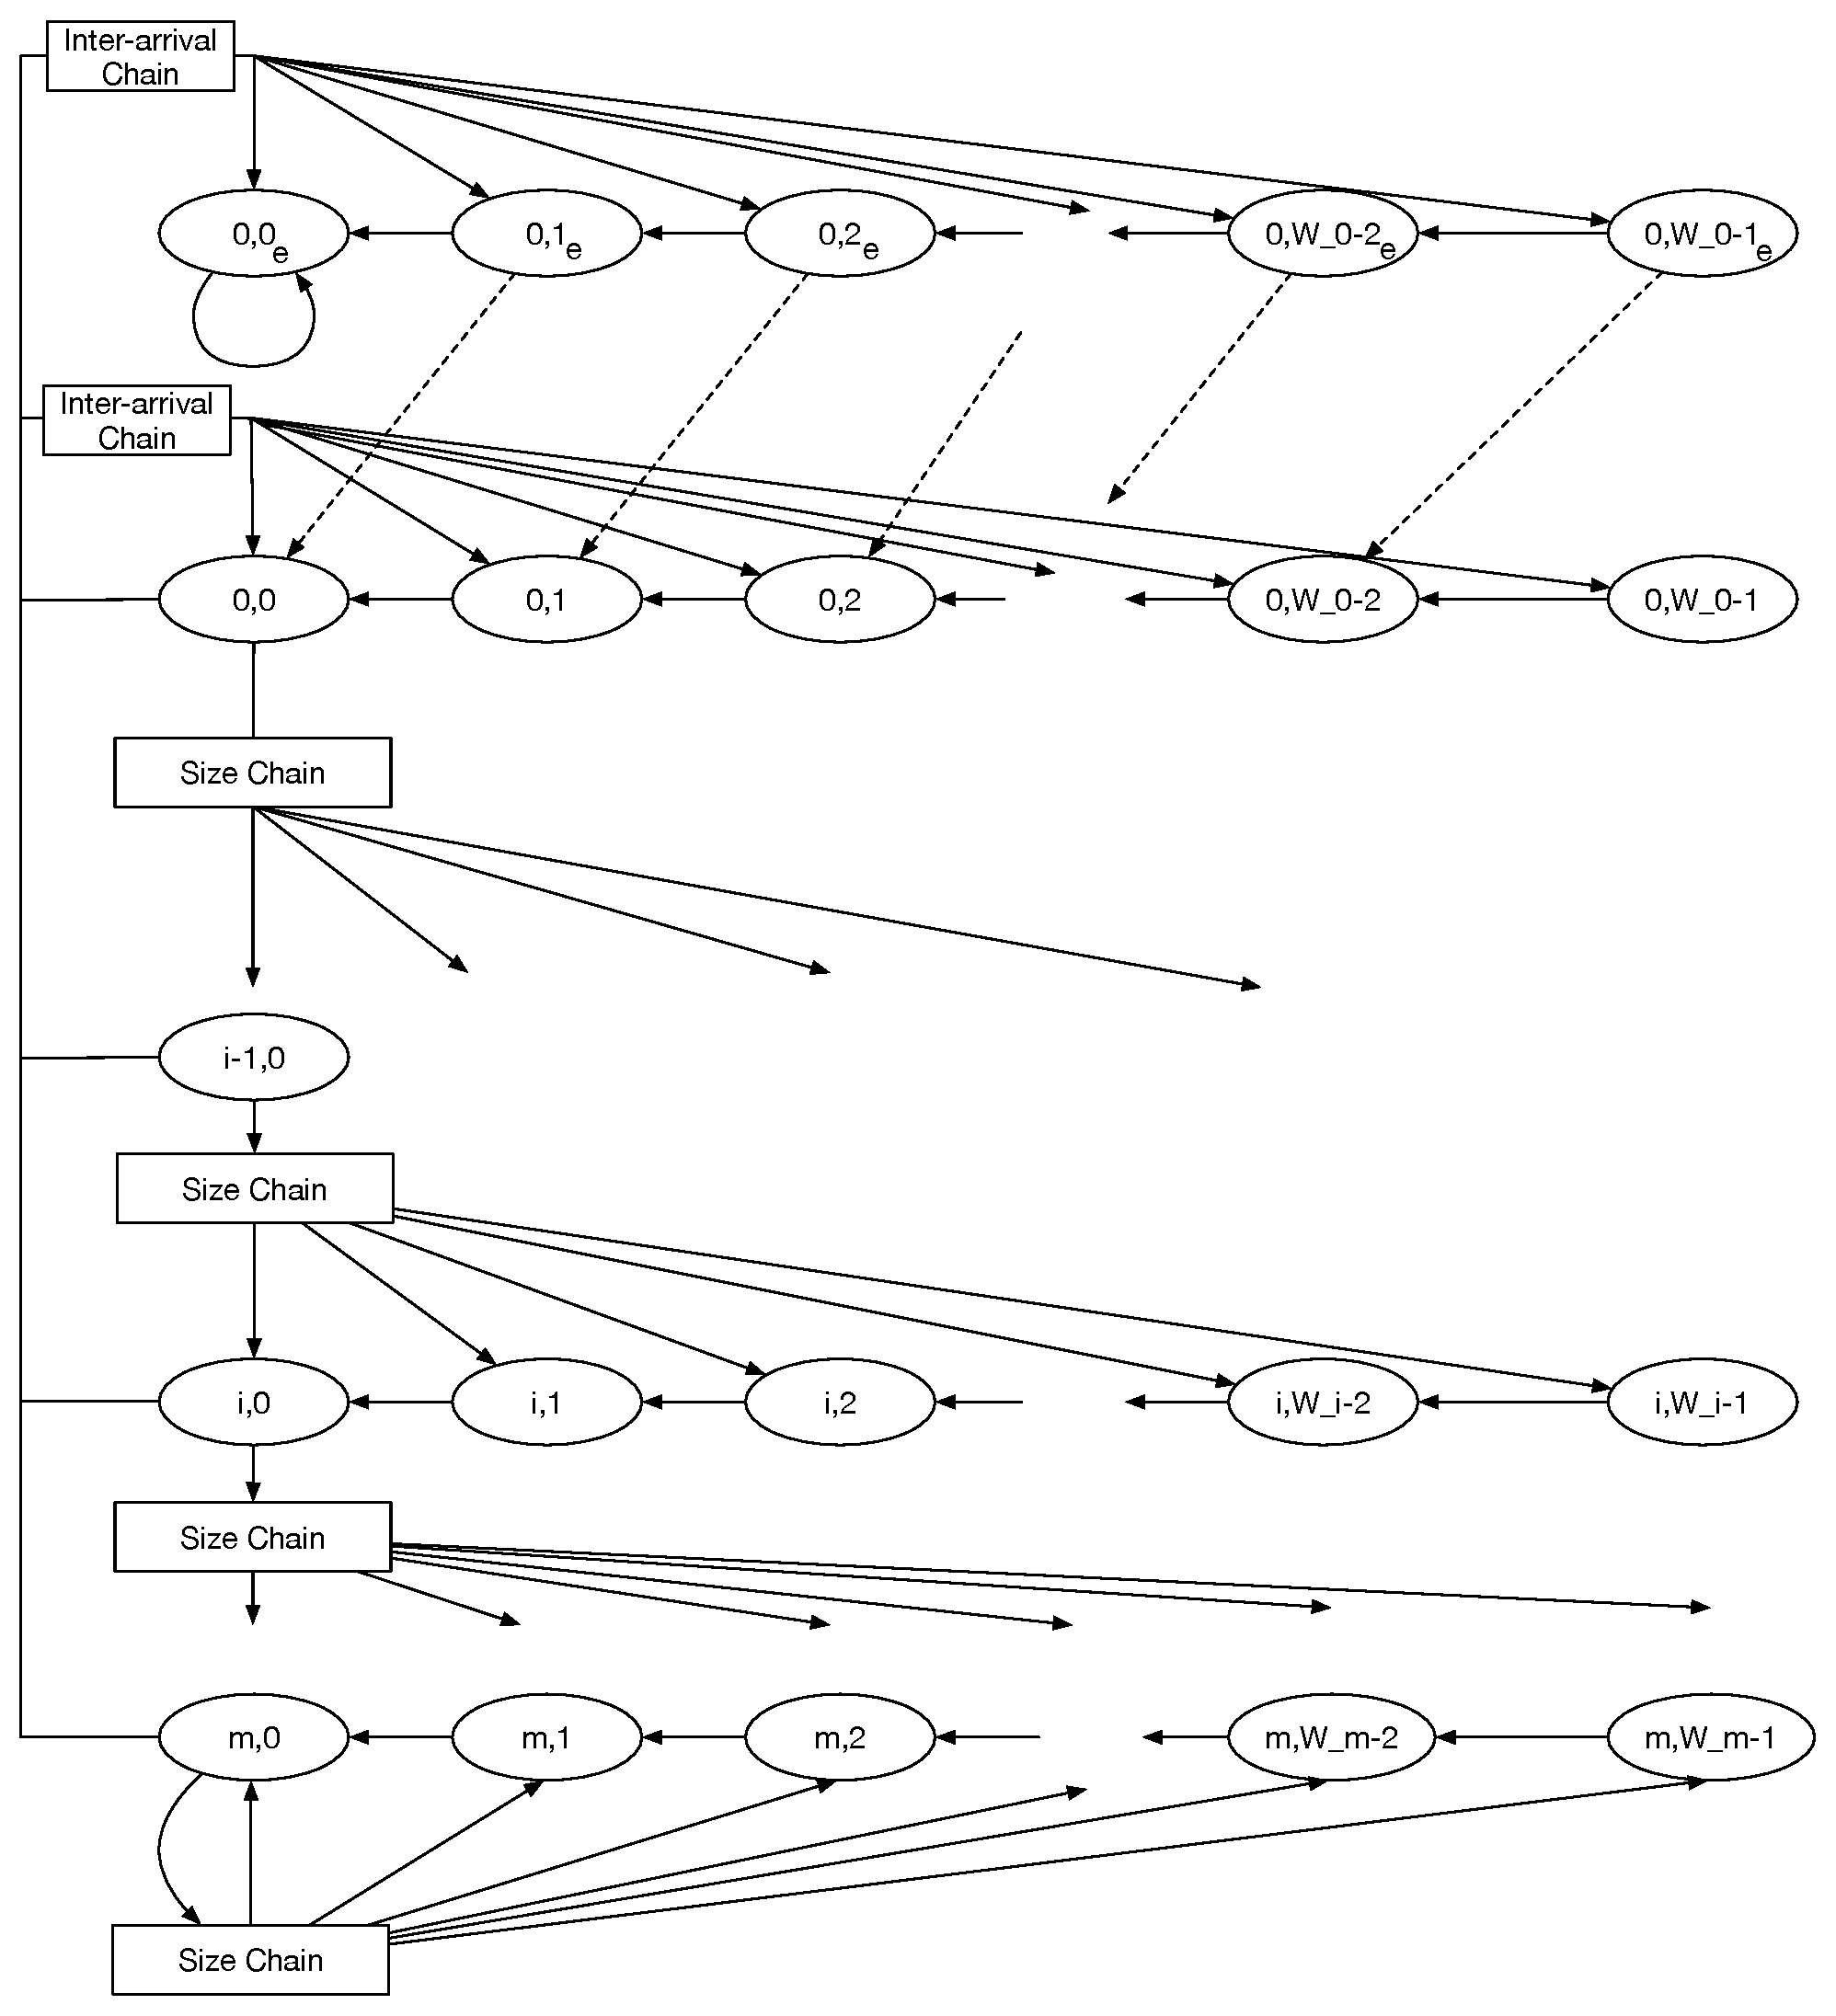
\includegraphics[scale=0.5]{../sketches/dcf_model_unsaturated_varpktsize_interarrival.pdf}
\caption{The modified unsaturated DCF Markov model that captures variable-length packet payloads.}
\label{fig:dcf_model_unsaturated_varpktsize_interarrival}
\end{center}
\end{figure*}

\bibliographystyle{IEEEtranS}
\bibliography{ref.bib}

% that's all folks
\end{document}
